% Note that because I talk a lot about binding ... this discussion within my methods section may be quite important for examing members that understands the physics but do not understand how MD simulations in particular is rigoroous enough to make any of those predictions.  Having those details here means that I understand how that link is established and that I'm not just making up stories based on pretty pictures.  These are some of the goals that I want to acheive for the benefit of the reader of this chapter.


% From D. Caplan's thesis - Molecular mechanics (MM) is the empirical mathematical representation of atomic inter- actions in the classical limit. MM was developed over 50 years ago and has been applied to organic chemistry as a tool to estimate specific energetic properties of small molecules. Since then it has evolved into various functional forms (known as �force fields�) used to describe the potential energy of a system by computing atomic interactions. Force fields may vary in the way that they represent atomic particles to balance experimental accu- racy with computational efficiency. Molecular dynamics (MD) is a MM-based method in which force fields are used to calculate the position, velocity, and acceleration of atoms over time to produce a trajectory.

\chapter[Methods]{Methods: Molecular Modelling and Simulation}

\section{Molecular Mechanics}
% Start by describing quantum mechanics 
% Assumptions and limitations of molecular mechanics
In principle, using quantum mechanics, the time-evolution of a molecular system can be predicted by solving the time-dependent Schr\"odinger's equation, which provides a complete description of the motion of atomic nuclei and electrons from first-principles.  REF However, the solution for this equation can only be obtained analytically for a hydrogen atom, and numerically using computational algorithms for very small systems. REF Many quantum-mechanics-based computational methods have been developed, but they are computationally prohibitive for probing biomolecular systems on a biologically-meaningful timescale because these systems typically possess on the order of 10$^{3}$ to 10$^{4}$ number of atoms. REF

\textbf{Molecular mechanics is an approach in which a molecular system is treated using the principles of classical mechanics.} In molecular mechanics, a molecule is modelled by a set of masses (atoms) connected by springs (bonds). REF An empirical potential energy function (PEF) that only depends on the positions of the atoms in the system is employed to describe the internal energy and interactions of molecules. REF The theoretical basis for molecular mechanics is rooted in quantum mechanics via the Born-Oppenheimer approximation. REF Under this approximation, the electronic and nuclear motion of atoms are considered to be uncoupled, \textbf{and therefore can be treated separately.} REF 
% Note that the previous sentence is a little vague -- what does it mean to be ``treated separately''
% This is because the nuclei, which are much heavier than electrons, are typically fixed on the time scales of electronic vibration. -- this sentence should be here because I need to make this logical connection before saying the next sentence
For this reason, the total energy (or the Hamiltonian, $H$) of a system can be considered to depend only on the electronic motion. 
% Although molecular mechanics is a very simplified model of molecular system, that made modelling of much larger biomolecular systems possible. 

The potential energy function employed in molecular mechanics corresponds to the Born-Oppenheimer energy surface of the molecular system in its electronic ground-state. REF In molecular mechanics, atomic nuclei are treated as point charges, where the motion of their electrons is implicitly accounted for in the PEF.  Because electronically excited states are not treated, no chemical reactions (i.e., bond formation) can occur.
% \cite{M. Born and R. Oppenheimer, Quantum Theory of Molecules, Ann. Physics, vol. 84, pp. 457�484, 1927.} -- can't find this article.
% \textbf{Say something good about MM approach}
\section{Force Fields}

The functional form of the potential energy function together with its associated parameters define a \emph{force field}.  A typical empirical force field has many parameters to be determined.  These parameters are typically determined by fitting to quantum mechanical calculations, and to physical measurements (e.g., using data from X-ray crystallography, neutron diffraction, vibrational raman spectroscopy) of small organic compounds or building blocks of peptides and nucleic acids.  Force fields are iteratively improved and extended by predicting experimentally observable quantities for small compounds, and adjusting parameters by comparing predicted quantities with experimental measurements.

In the past four decades, a variety of force fields have been developed for the purpose of modelling and simulating biomolecular systems involving peptides, proteins, nucleic acids and carbohydrates. Examples of the most widely adopted force fields include AMBER, CHARMM, GROMOS, and OPLS. REFs  Although each force field may vary slightly in the form of the PEF, most force fields utilize the general form:
\begin{equation}
\label{eq:ff_general}
	V = V(bonds) + V(angles) + V(dihedrals) + V(impropers) + V(non-bonded)
\end{equation}

\begin{figure}
 \centering
 \includegraphics[width=5in]{figures/methods/mm_schematic.pdf}
 \caption[A schematic of the representation of a molecule using molecular mechanics.]{A schematic of the representation of a molecule using molecular mechanics.}
 \label{fig:mm_schematic}
\end{figure}

\subsection{Bonded Interactions}
The first four functional terms of Equation~\ref{eq:ff_general}, $V(bonds)$, $V(angles)$, and $V(improper)$, describe the through-bond interactions covalent bond stretching, angle-bending, and bond rotations, respectively.  It is important to note that in molecular mechanics chemical bonds cannot be formed nor broken.  Covalent bond stretching can be described using Hooke's Law for harmonic motion,
\begin{equation}
\label{eq:bonds}
	V(bonds) = \sum_{bonds} k_b(b - b_0)^2.
\end{equation}

Likewise, angle-bending motions can be described harmonically as
\begin{equation}
\label{eq:angles}
	V(angles) = \sum_{angles} k_{\theta}(\theta - \theta_{0})^2. \\
\end{equation}

In Equations~\ref{eq:bonds} and \ref{eq:angles}, the constants $k_{b}$ and $k_{\theta}$ are the equilibrium force constants for bonds and angles, respectively, and the constants $b_{0}$ and $\theta_{0}$ are the reference bond length and angle, respectively. The total energetic contribution from bond stretching and angle bending are computed by summing over all bonds and angles in the system. In addition, the torsion (or dihedral) angle of bonds are also an important parameter in describing molecular conformations.  These energetic terms are commonly accounted for using a periodic function of the form,
\begin{equation}
\label{eq:torsion}
	V(dihedrals) = \sum_{dihedrals} \sum_{n} k_{\chi}(1 + cos(n\chi - \delta)),
\end{equation}
where $n$ denotes the periodicity of the rotational barrier, and $\delta$ is the reference angle.  Functions of this form (the so-called improper dihedrals) may be added to the PEF as a way of ensuring the planarity of planar chemical groups.


\subsection{Non-bonded Interactions}
Non-bonded interaction potentials predominantly account for van der Waals and electrostatic interactions.  Accurate reproduction of these interactions are particularly important for the transferability of a force field, that is, the ability to reuse a force field developed based on a set of molecule to predict properties of other molecules.  The non-bonded forces are only applied to atom pairs separated by at least three bonds. Van der Waals interactions are represented by the Lennard-Jones potential,

\begin{equation}
  \label{eq:lj_function}
  V_{LJ}(r) = \sum_{pairs} (\frac{r_{min}}{r})^{12} - 2(\frac{r_{min}}{r})^6.
\end{equation}

$V_{LJ}$ is a distance-dependent function that rapidly decays to 0 and represents a short-range attractive force. The first term of Equation~\ref{eq:lj_function} represents a repulsive force at distances where atomic shells overlap. The second term represents the attractive force between atoms which is most favorable at a distance of $r_{min}$, the preferred interaction distance for a pair of atoms.

The reproduction of electrostatics is paramount for describing interactions of polar and charged groups in biomolecules. To do so, an additive pairwise Coulombic potential is applied between all atom pairs which carry partial charges or charges at their nuclear centres.  This potential term, which depends on $r$, the distance between the pair of atoms, is given by

\begin{equation}
  \label{eq:electrostatic}
  V_{coulombic}(r) = \frac{q_iq_j}{\epsilon r}, 
\end{equation}
where $q_{i}$ and $q_{j}$ are the point charges on atoms $i$ and $j$, respectively, and $\epsilon$ is the the permittivity of vacuum.  In contrast to van der Waals interactions,  electrostatic interactions can be significant for charged pairs that are separated at longer distances. Accordingly, in comparisons to the Lennard-Jones potential, the Coulombic potential decays to zero at a much slower rate.

%\begin{figure}
% \centering
% \includegraphics[width=5in]{figures/methods/LJ_Coulumb_potentials.pdf}
% \caption[Lennard-Jones and Coulombic Potentials]{Lennard-Jones and Coulombic Potentials.}
% \label{fig:nonbonded_potentials}
%\end{figure}

As previously discussed in Chapter 1, hydrogen bonding is an important type of electrostatic interaction in biomolecular systems.  For this reason, a proper representation of hydrogen bonds should be captured by a force field. Some force fields have employed an explicit term solely for describing hydrogen bonding. For example, the original AMBER force field introduced in 1984 added a function of the form $\sum_{hbonds} C_{ij}/R_{ij}^{12} - D_{ij}/R_{ij}^{10}$ to account for hydrogen bonds.\cite{Weiner:1984uw}  However, it was later demonstrated that hydrogen bonding interactions are most accurately accounted for by appropriate parameterization of van der Waals and electrostatic potential terms. Hence, most modern force fields for protein simulations, including the latest AMBER force fields, no longer utilize an explicit hydrogen bonding term.
% Other things that I will not be discussing -- what were they again?

\subsection{Electronic Polarizability}
Polarizability is the measure of the change in a molecule's electron distribution in response to an applied electric field, and is a property of matter which can be induced by electrostatic interactions with solvents or ionic reagents.  As mentioned above, most current force fields use a fixed-charge model where each atom in the system is assigned a single value, which remains independent of changes in its local electrostatic environment. Next-generation force fields have been proposed to  incorporate models for electronic polarizability. REF However, because of the associated prohibitive computational cost with the use of these force fields, they are not currently widely used for biomolecular simulations.
% The introduction of polarizable force fields into common use has been inhibited by the high computational cost associated with solving this problem self-consistently.

\subsection{The AMBER and OPLS Force Fields}
In this section, I briefly describe two widely used popular force fields for protein simulations, AMBER and OPLS. The OPLS-AA and AMBER99 versions of these force fields were employed in the studies presented in Chapters 3 to 5, and 6, respectively.  More extensive and detailed reviews of empirical force fields for biomolecular simulations have been provided elsewhere.\cite{Ponder:2003uw,MackerellJr:2004p5558}

One of the first force fields for the simulations of proteins was the AMBER force field, which was developed in the Kollman group.\cite{Weiner:1984uw}  The central ideas for parameterization was to fit atomic point charges to the quantum electrostatic potential (ESP) using \emph{ab initio} quantum mechanical calculations, and develop parameters for the bonded and  van der Waals potential terms using experimental structural data and liquid-state simulations. The initial parameters were improved upon via the reproduction of experimental measurements for model compounds. The AMBER force field was initially develop by only accounting for non-aliphatic hydrogen atoms.\cite{Weiner:1984uw}  An all-atom version of AMBER was developed in 1995.\cite{Cornell:1995td} Since then, many iterations of improvements upon the original all-atom AMBER force field have been developed. In particular, AMBER99 (or ff99) is one such revision with newly developed parameters to improve the reproduction of protein secondary structure.\cite{Wang:2000uu}

%The potential energy function for AMBER is as follows: 
%\begin{equation}
%\begin{split}
%V = \sum_{bonds} k_b(b-b_0)^2 
%   + \sum_{angles} k_{\theta}(\theta - \theta_{0})^2 \\
%   + \sum_{dihedrals} k_{\chi}(1 + cos(n\chi - \delta)) 
%   + \sum_{impropers} k_{\gamma}(\phi - \phi_{0})^2 \\
%   + \sum_{nonbonded} \frac{q_1q_2}{er} \\
%   + \sum_{nonbonded} \epsilon [(\frac{r_{min}}{r})^{12} - 2(\frac{r_{min}}{r})^6]
%\end{split}
%\end{equation}

OPLS, short for optimized potentials for liquid simulations, was originally developed to simulate and reproduce liquid state properties, such as the densities and heats of vaporization of neat organic liquids.
 These potential functions were first developed for water, ions and hydrocarbons,\cite{Jorgensen:1984vy} and then was later extended to amides and peptides.\cite{Jorgensen:1985wx} The non-bonded interactions in OPLS were derived by comparisons to liquid-state thermodynamics. Like AMBER, in early OPLS development, a partial united-atom model was used whereby nonbonded interaction sites were placed only on non-hydrogen atoms and polar hydrogens.\cite{Jorgensen:1988vg,Jorgensen:1985wx,Jorgensen:1984vy}

An all-atom OPLS force field (OPLS-AA) for organic molecules and peptide simulations was developed in 1996.\cite{Jorgensen:1996vx} Although the parameters for charges and van der Waals interactions were developed from simulations of pure liquids, which is unique to the parameterization methodology of OPLS, the atom types and parameters for bonded interactions (bonds, angles, and dihedrals) were largely adopted from the AMBER all-atom force field.\cite{Jorgensen:1996vx}


\section{Molecular Dynamics Simulation}
% Approximations made in MD.
% Note the audience of your thesis.  It is good to cover basic ground.  I think I should also brief talk about enhanced techniques.
At a very high level, MD simulation is an algorithm to simulate motion of a system under the influence of a specific force field by following molecular configurations in time according to Newton's equation of motion. 

% This is the part with the time propagation using the Equations of motion
In a system of $N$ interacting particles, the force on each particle in the system is determined by taking the spatial derivative of the potential energy of the system, $V(r_{1}, r_{2}, ... , r_{N})$.  In MD simulations, this potential energy is approximated by a molecular mechanics force field as described above.  The force on each particle $i$ is given by
% Not exactly ... according to Chris Madill's thesis, U is the potential energy between an atom pair?  Clear up the core algorithm!
\begin{equation}
% F_i = - \nabla U
  F_i = - \frac{\partial V}{\partial r_i}, i = 1, 2, 3, ... , N.
\end{equation}

The variable $r_{i}$ represents the spatial coordinates of the particle $i$. The calculated force vectors are summed together to yield the net force vector acting on every atom in the system. By Newton's second law of motion, the acceleration, $a_i$, of each atom is given by 
\begin{equation}
a_i = \frac{F_i}{m_i},
\end{equation}
where $m_i$ is the mass of the $i$th particle. Hence, the position of atom $i$ at time $ t + \delta t$ is then
\begin{equation}
x_i(t + \delta t) = x_i(t) + v_i(t)\delta t + \frac{a_i(t)\delta t^2}{2}  
\end{equation}

To determine the positions of each of the $N$ particles requires solving a system of 3$N$ differential equations.  Such a system of differential equations can only be solved numerically, and in MD simulations, a time-integration algorithm is typically employed. REF Once the position of each particle is computed, interatomic forces are updated based on these new coordinates, and the entire process is repeated to obtain the coordinates of the system for subsequent time steps. To ensure numerical stability, a small integration time step in the range of 1 - 4 femtoseconds (fs) is chosen. REF Typically, in a MD simulation of a biomolecular system, a 2 fs timestep is used as it is twice the time period for the fastest vibrational motion (existing in bonds involving hydrogen). REF % [Ref: Chris Madill's and Tom's thesis]

% There are many different forms of integration algorithms, with the most common being the Verlet and leap-frog algorithms. 
% According to gromacs manual:
% md - is a leap-frog algorithm for integrating Newton's equation.
% Note that in absence of pressure and temperature coupling, verlet and leap-frog is equivalent ... and generates identical trajectories of motion.

% How much detail? Talk about the velocity verlet integration algorithm ? -- I'm going to study up on this but will eliminate this from my thesis ...


% Marty's thesis included a little bit on the verlet algorithm.  CN did not.

\subsection{Temperature and Pressure}
% My goal is to describe how temperature and pressure coupling is handled in MD at a high-level without going into the details of the math.
% Ref: Understanding Molecular Simulations by Frenkel Daan.
The inclusion of temperature in MD allows for the account of entropy in our systems, which is especially important for free energy determination. The theorem of equipartition of energy states that in a (classical) many-body system at thermal equilibrium, the average kinetic energy (KE) per degree of freedom is related to the thermodynamic temperature, $T$, via 
\begin{equation}
  KE_{avg} =   \frac{1}{2} k_BT,
\end{equation}
where $k_{B}$ is the Boltzmann constant. In MD simulations, the temperature of the system is determined by calculating the total kinetic energy of the system and normalizing by the number of degrees of freedom in the system, $N_{r}$.  The instantaneous temperature of the system is 

\begin{equation}
  T(t) = \sum_{i=1}^{N} \frac{m_iv_i^2(t)}{k_BN_f}.
\end{equation}
where $N$ is the number of atoms in the system. To simulate a system under comparable laboratory conditions,  a thermostat and a barostat (a virtual pressure piston) are employed in simulations to control both temperature and pressure, respectively.  Several of these temperature- and pressure-coupling algorithms exist, and they are reviewed in detail elsewhere. REF 
% These algorithms have been validated to produce the correct statistical mechanical ensemble averages.  
%\cite{[25] Nose ́, S. A molecular dynamics method for simulations in the canonical ensemble. Mol. Phys. 52:255–268, 1984.[26] Hoover, W. G. Canonical dynamics: equilibrium phase-space distributions. Phys. Rev. A 31:1695–1697, 1985.}

%Below is from the GROMACS manual:
% While direct use of molecular dynamics gives rise to the NVE (constant number, constant volume, constant energy ensemble), most quantities that we wish to calculate are actually from a constant temperature (NVT) ensemble. 
% Using the same idea, we can couple the system to a pressure bath.  This method is called the Parrinello-Rahman pressure coupling, and the theory has been shown to correctly produce the NpT ensemble.
% \cite{Parrinello, M., Rahman, A. Polymorphic transitions in single crystals: A new molecular dynamics method. J. Appl. Phys. 52:7182–7190, 1981. [35] Nose ́, S., Klein, M. L. Constant pressure molecular dynamics for molecular systems. Mol. Phys. 50:1055–1076, 1983.}
% Should I include the equations? I haven't seen this in other thesis, perhaps its too much detail. -- Yes this is too much detail.

%\subsection{Solvent Representation}
%% Talk about how solvent is accounted for
%The most realistic simulations treat the solvent environment by explicitly including the water molecules.  \textbf{How solvents are parameterized.  Can mention a few details about TIP3P water model. I actually don't know much about TIP3P} Solvent models are chosen to be consistent with the force field used for modelling the protein.  Although using explicit solvent leads to the most realistic simulations, these simulations are computationally expensive.  In some cases, instead of using explicit solvent molecules, implicit solvation can be used, that is the presence of solvent is approximated by using a potential. However, the implicit solvation suffers from several key weaknesses including a poor description of water-mediated interactions, directionality of water hydrogen bonds and only an approximate treatment of the nonpolar contribution to solvation.
%Hence,  is much less accurate and can introduce force field inconsistencies leading to inaccurate results.\cite{Yang:2013ff}

\subsection{Periodic boundary conditions}
Periodic boundary conditions (PBC) is a technique by which the central simulation cell (or ``box'') is replicated along each of its dimensions to form a system with infinite number of images.  PBC is used in MD simulations to alleviate artificial phase boundaries which are imposed by a finite simulation cell.  Furthermore, PBC allows the system to be treated as a bulk system, akin to that of an \textit{in vitro} experimental system.  To avoid counting duplicate interactions from multiple adjacent cells, an atom $i$ interacts with only another atom $j$, provided that $j$ is in $i$'s closest periodic images. Because of this constraint, care must be taken to chose a central box size large enough to avoid artificial interactions induced by periodic boundaries. REFS

\subsection{Theoretical Basis of MD Simulations}
MD simulations yield information about the microscopic states of a macroscopic system characterized by thermodynamic variables such as temperature, pressure, the number of particles, free energy, etc.   Thermodynamic variables are what is typically observed and measured experimentally.  Statistical mechanics is a body of theory that provides a rigorous connection between the microscopic arrangements of a system (determined by MD simulations) to its thermodynamic properties.
 
For an ensemble of microstates, the probability of finding a system in the microstate $i$, with an energy $E_{i}$ is given by the Boltzmann distribution,
\begin{equation}
p_{i} = \frac{1}{Z}e ^{\frac{-E_{i}}{kT}}.
% Z = e ^{\frac{-A}{k_{B}T}}
\end{equation}
$Z = \sum_{i} e ^{\frac{-E_{i}}{kT}}$ is the normalization factor (or the \emph{partition function}) so that $\sum_{i} p_{i} = 1$.

MD simulations can be carried out in the canonical (NVT) or  isothermo-isobaric (NPT) ensembles, where the average pressure of the system is held constant and the volume of the simulation is allowed to fluctuate. Because the NPT ensemble is the closest to experimental conditions, production simulations are often carried out in this ensemble.

Given the partition function, one can then determine any thermodynamic variable. For example, free energy is an important thermodynamic quantity which measures the useful work obtainable from a system under a certain set of condition.  This quantity is called Gibbs free energy (G) and Helmholtz free energy (A) for a system in the NPT and NVT ensembles, respectively. In biochemistry, a central quantity is the change in free energy between two states, which measures whether a reversible biochemical process will occur spontaneously.  $\Delta G$ for any two states, 0 and 1, is related to their respective probabilities $p_{0}$ and $p_{1}$ by

\begin{equation}
\Delta G = - k_{B}Tln(\frac{p_{0}}{p_{1}}).
\end{equation}

Performing an MD simulation yields a time-trajectory of motion of the molecules in the system from which we can obtain time-averaged properties of the system.  However, in an experiment, the macromolecular observables measured are a result of an average of all possible system configurations, or an \emph{ensemble average}.  This apparent conundrum is reconciled by one of the fundamental axioms of statistical mechanics, the ergodic hypothesis, which states that if a system is given long enough time to evolve, the time average of its macromolecular properties is equivalent to their ensemble averages.  In practice, this means that if a MD simulation sufficiently samples the relevant regions of the phase space of the system of interest, then experimentally-relevant properties may be calculated from such a simulation.

\subsection{Enhancing Sampling of Biomolecular Simulations}
As described above, in an MD simulation, atomic motion is dictated by a potential energy function, and states are sampled with probabilities dictated by the Boltzmann distribution. Given an infinite amount of time, a simulation will sample all thermally-accessible states of a system's potential energy landscape. However, such infinitely long simulations are not possible to achieve computationally feasible, and due to the rugged energy landscapes common to biomolecular systems, many important states may not be sampled on the timescales of a typical simulation.
Furthermore, it is even more challenging to adequately sample the complex conformational landscape of disordered proteins because potentially many thousands of conformational states must be sampled in order to fully characterize their structural ensemble [4].

Generalized-ensemble algorithms are a class of algorithms that can be used with molecular simulations to enhance conformational sampling.  Simulated tempering (ST) and replica exchange (RE) are two well-known generalized-ensemble algorithms that can be used to enhance sampling by allowing simulations to diffuse in temperature-space, while obeying Boltzmann statistics. These algorithms rely on the underlying assumption that at higher temperatures the free energy landscape of a biomolecular system becomes less rugged, and, hence, the crossing of energetic barriers are facilitated.  A temperature range is typically chosen to include temperatures lower and higher than the room temperature (300 K), and is dependent on the size and composition of the system.  Although generalized-ensemble methods can greatly enhance sampling, they can be computationally very expensive to carry out, and can, in some cases, require hundreds of compute nodes to run simultaneously for many months to complete a single study.  

In Chapters 3 and 4 of this thesis, the ST algorithm was used to generate the structural ensembles of (GA)$_{4}$ and A$\beta$(16-22) peptides.

%\subsubsection{Approaches for Determining Protein Conformational Ensembles}
%It was mentioned in Chapter 1 that enhanced sampling may be used to speed up simulations.  Here we provide a high level overview of the approaches that were developed that have been useful in sampling of peptide and protein conformations in molecular simulations. 
%
%The use of temperature to overcome energetic barriers in the system. Here I can talk about what enhanced sampling is, and how they can be applied to understanding the properties of disordered peptides. Cite Sarah.  
%I should read both Sarah's and Chris's thesis chapters relating to sampling.  Chris's is all about sampling. Since I refer extensively to enhanced sampling, I should make a mention of it.
%
%\subsubsection{Approaches for Calculating Protein-Ligand Binding Affinities}
%Note: This section could actually be put in the introduction.  As this may not require understanding the details of simulations.  Leave this hear for now and can move it as a section to the introduction ... maybe after Regis has seen both chapters together.
%
%I can show the thermodynamic cycle for getting Delta G, like the one that I had in my transfer proposal.  Describe why this can be used to determine free energies.  And then mention the techniques that were invented in the past to do so. These approaches are not applicable to the problem of this thesis, but this background is provided to give the reader perspective. Point to another review article and say this is discussed in detail. I can discuss how to determine enthalpic and entropic contributions.


%\subsection{Better Hardware}
% Here can describe how better hardware - bigger and better machines have led to improvements and advancements in this field.

% Initial conditions -- initial positions of the atoms in the system

\section{Practical Aspects of Preparing a Biomolecular System for MD Simulation}

Coordinates for the initial input into a simulation software need some care to be prepared.  First the structure of protein or peptide to simulated need to be generated.  The starting structure of the target protein is usually X-ray crystal or NMR structure, which can be taken from the Protein Data Bank.  Then the simulation environment is prepared to closely mimic the experimental conditions (usually experimental crystallization conditions). For example, the pKa of a protein is typically predicted so that residues such as histidine are appropriately protonated.

For a simulation of a globular protein, after the protein structure has been prepared, cosolutes, salt and water molecules are added to create the final simulation box. However, for more complex simulation systems, such as those in the presence of a lipid bilayer, additional steps
% Also make sure that at this point everyone in my committee understands that there is no ionization in the simulations and no chemical reactions.  
 
At this stage,  an energy minimization algorithm is usually performed on the system to correct any bad steric contacts that might have been introduced when solvent was added. An example of a completed starting structure of a simulation is shown in Figure~\ref{fig:simulation_box}.

\begin{figure}
 \centering
 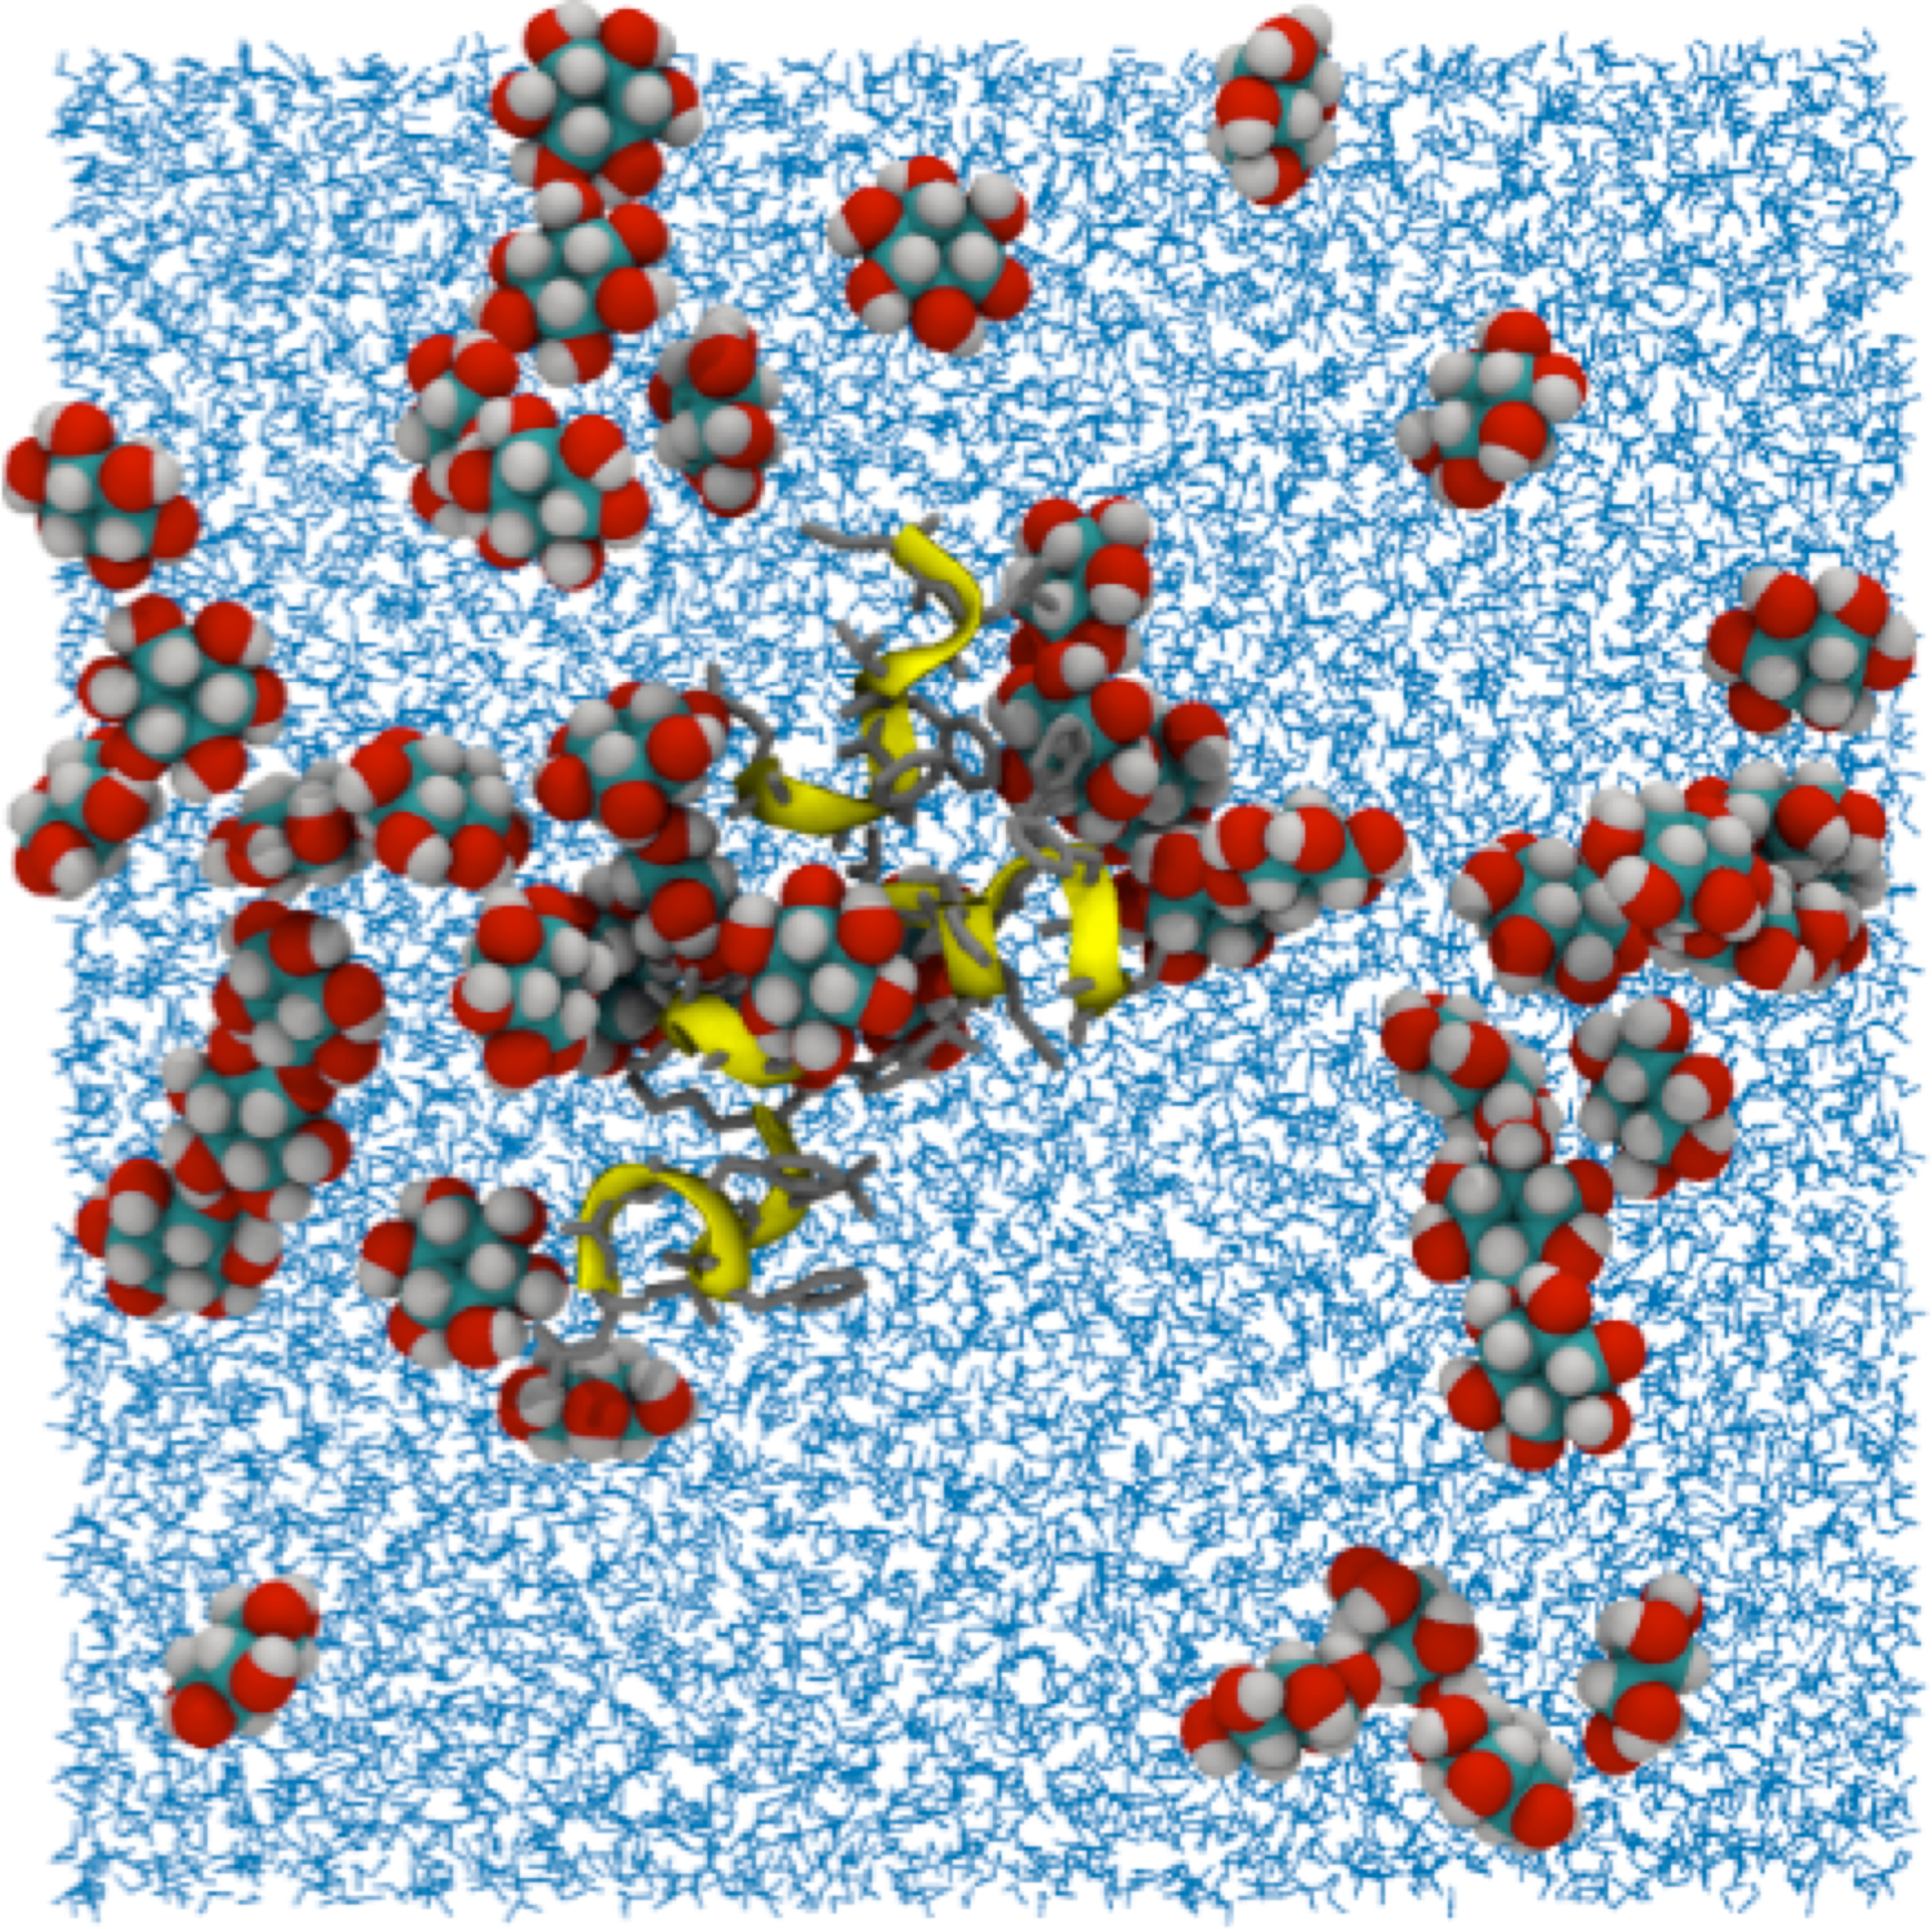
\includegraphics[width=5in]{figures/methods/simulation_box.pdf}
 \caption[An example of a MD simulation system]{An example of a MD simulation system.}
 \label{fig:simulation_box}
\end{figure}

Prior to performing production dynamics, which is what most of the results from a simulation will be based on, a short simulation to equilibrate the system is performed.  Equilibration is performed to allow the pressure and temperature of the system to stabilize. Here the stability of the protein is also validated to ensure that the protein structure has not grossly deviated (or unfolded) from the starting model.  

\begin{figure}
 \centering
 \includegraphics[width=5in]{figures/methods/equilibration.pdf}
 \caption[RMSD from the initial crystal structure calculated from an equilibriation]{Equilibration of the simulation system.}
 \label{fig:simulation_equilibration}
\end{figure}

\addcontentsline{toc}{section}{Bibliography}
\bibliographystyle{plain}
\bibliography{introduction}

%\section{Application of MD in structure-based drug discovery}
%
%% \1 (Why computational?) Can help us get protein dynamics is important for understanding protein function. We want to understand protein function because we want to be able to design drugs to cure diseases.
%
%% \1 A important application of MD simulation in biochemistry is the predicting of protein-ligand binding free energies.
%
%One application of MD simulations is in rational drug design. In recent years structure-based computer modeling of protein-ligand interactions have become a core component of modern drug discovery.  In early stage drug discovery, a target is identified along with putative binding sites.  Then, the structure of the target is determined using structural determination techniques such as NMR or X-ray crystallography.
%% [See Tom's thesis]
%Ligands which may act as potential drugs are expected to bind with a high affinity (low $K_d$) to the binding site. The goal is to discover,  high specificity inhibitors of a protein (usually an enzyme). In this process, the binding free energy of the ligand to its target is used to quantitatively evaluate how well a ligand binds. A crude estimate of the binding affinity can be obtained using computational docking methods, where the energetics of binding is typically estimated without accounting for either ligand or protein flexibility.  Although docking is fast, it is often inaccurate for identifying true drug candidates.
%
%With computer hardware becoming faster and cheaper, MD simulations can be used to rapidly prototype experimental ideas -- for example, one can perform computational alchemy, that is, ``mutate'' residues to test various hypotheses. Furthermore, simulations may be used to determine whether a chemical change will produce a more potent drug candidate. Currently, state of the art computational binding studies use MD simulations, where the protein and drug is allowed to relax and freely move about in the system. However, in the case of understanding a specific binding reaction often needed when developing an enzyme inhibitor, the ability to observe the relevant binding events is a low probability event on the timescale achievable by simulations. Therefore, a few enhanced techniques have been developed to accelerate this process.  They are briefly introduced below.
%
%\section{Free energy calculations}
%There are two advanced methods that have been developed for determining the absolute binding free energies in combination with MD simulations.
%
%% \3 Linear interaction energy -- Out of scope
%% \3 MM/PBSA - no explicit account for solvents -- Out of scope
%\subsection{Thermodynamic perturbation}
%This is the paper that I am taking most of the topics here\cite{Gilson:2007hz}
%
%\subsection{Thermodynamic integration}
%I actually have no idea what this is, and would be hard pressed to explain this properly.
%In this case, I don't think I should be covering these topics in my thesis.
%
%\subsection{Free energy perturbation}
%Alchemically change one molecule into another
%
%\section{Review of MD studies of amyloid inhibition by small molecules}
%% MD studies using brute-force sampling. Aid in medicinal chemistry by making suggestions for how to design new AD drugs.
%
%\begin{outline}
%	%  Excerpt from Transfer proposal
%	\1 In recent years, molecular dynamics simulations have been intensively used to investigate the molecular basis of the structure and stability of amyloid fibrils. 
%	
%	\1 MD simulations of Congo red binding have been done with the protofibril-like crystal structure composed of the segment GNNQQNY.\{Wu, 2007 \#621\}
%	
%	\1 A recent simulation study of an N-methylated peptide with A$\beta$16-22 models of amyloid aggregates has provided insight into the possible mechanism of action of peptide inhibitors of amyloid formation.\{Soto, 2007 \#597\} This peptide inhibitor was shown to preferentially bind monomers to form dimers, possibly acting to inhibit fibril formation by sequestering monomers. However, peptide-based inhibitors have poor pharmacological profiles as they are actively broken down by proteases in the stomach and are difficult to transport across the blood-brain barrier. In addition, these peptide inhibitors specifically target A$\beta$ and thus do not have the potential to treat multiple amyloid diseases.
%\end{outline}


% Scrap
% Motivate the use of MD simulations
% Describe the details of molecular dynamics simulations
% Review the basic derivations of MD simulation equations and why they work

% Molecular dynamics simulations are a useful tool to study the structure, dynamics, and interaction of biomolecules. 

% MD is a numerical algorithm which solves a system of Newtonian equations of motion, and provides as output the time-trajectory of atoms with femtosecond time resolution.

% To review before my defense

% Details of the mathematics (need to review the basic theory + Taylor series expansion) - get a book - tomorrow maybe?

% Why is MD correct? Describe the fundamental assumptions of MD. Here, I want to give the readers who aren't familiar with the methodological details of MD a sense of the rigorousness of MD.

% The assumption at a hand-wave level adapted from Tom's thesis

% - Relationship between force and energy 
% - Relationship between momentum and velocity 
% - Why numerical approach must be used (no analytical solution for N > 2)
% - How is the force field plugged into the general algorithm.






% \subsection{Setting up a MD simulation: practical aspects} - Here are some details to run a MD simulation of a biomolecular system.  Should I omit this from my introduction? This is not really essential in understanding the rest of my thesis, or is it? Perhaps this should go into an appendix instead -- this isn't interesting. The following steps are often used to setup and start a MD simulation system of a protein. First, a pre-determined structure, typically a coordinate structure from X-ray crystallography or NMR, or homology-modelling data. Then a force field and solvent is chosen.


%\section{Limitations of MD simulations}
% Rauscher:2010p5682,Rauscher:2009wr}  % Ref: DE Shaw and CN
% Schlick T (2010) Molecular modeling and simulation: an inter- disciplinary guide, interdisciplinary applied mathematics, vol 21, 2nd edn. Springer, New York


% Given the approximations of MD, MD is well-suited for probing the dynamics of complex systems on the timescale of picoseconds to seconds. ???

%Roughly speaking, one would like to run a simulation at least 10 times longer than the slowest important timescale in a system. Unfortunately, many biomolecular timescales exceed 1 ms, and in some cases by orders of magnitude (44).\cite{Zuckerman:2011dz} For molecular simulations to reliably predict, guide, and help explain experiment, these simulations require force fields of sufficient accuracy, adequate sampling of the relevant biomolecular motions (convergence) and a correct representation of the experimental conditions. Failures in any of these areas yield results which disagree with experiment.Until sampling is adequate, equilibrium properties computed from a simulation remain biased by the system�s starting state and no meaningful comparison with experiment is possible [6]. 

%% copied from Zukerman\cite{Zuckerman:2011dz}
%\textbf{Although routine explicit-solvent MD simula- tions are now four or five orders of magnitude longer (i.e., 100-103 ns currently), modern MD studies still appear to fall significantly short of what is needed for statistically valid equi- librium simulation (36, 38). Roughly speak- ing, one would like to run a simulation at least 10 times longer than the slowest impor- tant timescale in a system. Unfortunately, many biomolecular timescales exceed 1 ms, and in some cases by orders of magnitude (44).}
%% Other references that are relevant for sampling \cite{Grossfield:2009bn}
%
%% Copied from \cite{Mobley:2011ks}
%\textbf{For molecular simulations to reliably predict, guide, and help explain experiment, these simulations require force fields of sufficient accuracy, adequate sampling of the rel- evant biomolecular motions (convergence) and a correct representation of the experimental conditions. Failures in any of these areas yield results which disagree with experiment. 
%
%We may be tempted to blame disagreement with experiment on just one of these areas�force fields are perhaps the most common scapegoat, sometimes with good reason [1�5]�but any or all of the three may be a weak point. And, in some sense, adequate sampling is the weakest link. 
%
%Until sampling is adequate, equilibrium properties computed from a simulation remain biased by the system�s starting state and no meaningful comparison with experiment is possible [6]. 
%
%With an inadequate force field or a poor representation of the experimental conditions, results will disagree with experiment, but will be robust and improvement is relatively easy, but not so with inadequate sampling.}
%
%% copied from Sarah's thesis
%\textbf{Achieving complete (or even adequate) conformational sampling is one of the key challenges in biomolecular simulations.\cite{Gnanakaran:2003vh} The energy landscape of most biomolecules is �rugged� and the source of this ruggedness is two-fold. The energetic barriers separating accessible states are often larger than the available thermal energy, and there are typically a large number of states to be sampled. The timescales of many biomolecular processes, such as protein folding, are still far beyond the reach of our current computational capability, which is generally limited to the 10-8-10-7 s timescale for continuous simulations. For example, even the folding of small domains or secondary structure elements, such as ?-hairpins and mini-proteins, occur on the 1-10 ?s timescale.1 
%
%Consequently, conventional or �brute force� molecular dynamics (MD) alone is often insufficient to achieve complete Boltzmann sampling of the important states of many biologically relevant systems. For this reason, generalized-ensemble algorithms have become popular tools for conformational sampling.}

% Topics that I'm not going to discuss
%Evaluating the convergence of simulations is still a challenge - I don't want to  go into this as this is out of the scope of my thesis.
%Limitations in the accuracy of current force fields - Don't talk about this .. but this will probably come up during the defense regardless.